\documentclass[12pt]{article}

\usepackage{url} % websites in bib
\usepackage{hyperref}
\usepackage[a4paper,left=1in,right=1in,top=1in,bottom=1in]{geometry} % margins
\usepackage{paralist} % compact enumerates

\usepackage{graphicx}
\usepackage{caption}
\usepackage{subcaption}

\usepackage{amsmath}

\usepackage{todonotes}

\begin{document}
	\title{Software project: K-Means Improvements}
	\author{Stefan Sebastian, 242}
	\date{}
	\maketitle
	
	\newpage
	\tableofcontents
	\newpage
	
	\section{Specification}
	The purpose of this report is to document the 'K-Means Improvements' software library. The project presented contains implementations for the basic K-Means algorithm with random seeds and some improvements in terms of computation speed (Enhanced K-Means) and seed selection (K-d trees density based, Sort and split heuristic). The library offers some clear, easy to use methods for performing clustering and can be extended to incorporate new algorithms by following some simple conventions.
	
	\subsection{Motivation}
	The amount of data available is growing at an explosive rate\cite{HowMuchDataDoWeCreateEveryDay} and most of it comes from people interacting online and does not have meaningful labels. There is a need for computationally efficient and reliable clustering methods and it does not make sense for every researcher to implement them in order to do an experiment. Furthermore, a good knowledge of algorithms might not be among the skills of a data scientist, meaning that they will look for a suitable tool. 
	
	Most frameworks that are popular in the python environment (sk-learn, tensorflow, etc) offer a wide selection of algorithms from different artificial intelligence subfields. Thus, it is not reasonable to expect that each topic will always be up to date with research results. This framework is narrow in scope, only considering K-Means clustering, meaning it can cover a wide range of improvements and variants from recent years.
	
	\subsection{Theoretical background}
	The first version of the library contains the following algorithms: basic K-Means, Enhanced K-Means, seed selection with K-d trees, seed selection using the Sort and Split heuristic. This section will give an overview of those algorithms and the context in which they are useful.
	
	\subsubsection{Enhanced K-Means}
	A simple improvement for the basic K-means has been proposed by Fahim et al.\cite{EfficientEnhancedKmeans} under the name of "enhanced K-means" in 2006. The main idea is that some time can be saved during the computation of distances between points and cluster centers in the update phase of the original algorithm. This distance is calculated at every iteration of the algorithm but the information from previous iterations could be used, by employing an additional data structure that memorizes the previous distance between a point and its cluster's center. At every iteration the distance to the new cluster mean is calculated and if it's less or equal to the previous distance stored for that point then it is left in its cluster and there's no need to calculate the other k-1 distances.
	
	The complexity of this algorithm can be approximated to O(nk) compared to the complexity of the classic algorithm which is O(nki), where n represents the number of points, k the number of clusters and i the maximum number of iterations. In brief, the time complexity when updating the position of a point is O(1) if it stays in its cluster and O(k) otherwise. Since the algorithm converges to a local minimum then the number of points updated in each iteration decreases, meaning the expected complexity is \( nk\sum_{j=1}^{i}1\mathbin{/}j \).
	
	\subsubsection{Seed selection using the Sort and Split heuristic}
	This conceptually simple heuristic for choosing the K-means seeds was proposed by Yedla et al.\cite{SortSeed} in 2010. The main idea of the method is to sort all points in the initial dataset by distance from origin. In case that there are points with negative feature values then they are transformed, by subtracting the minimum attribute value out of the feature value for each point. After sorting, the data is partitioned in k equal sets, where k is the number of desired seeds. From each set, the middle point is chosen as a seed. This method was compared to the classic algorithm that uses the random seed initialization and has been shown to obtain better accuracy on all testing sets.
	
	\subsubsection{Seed selection with K-d trees}
	A k-d tree, introduced by Jon L. Bentley\cite{KdTree}, meaning k-dimensional tree is a data structure used to organize points in k-dimensional space, which is useful for partitioning data and optimizing multidimensional queries.
	
	An implementation of seed selection based on the k-d structure is proposed by Redmond and Heneghan\cite{KdTreeKmeans} in 2007. The reason for using this data structure is to gain information about the density of the dataset. In order to suit the problem some decisions have been made while building the tree. At each step the dataset is split among the longest dimension of the bounding box. This box can be computed by taking the minimal and maximal values for each feature in the dataset, and building two new points. The longest dimension is simply the feature for which there is the greatest difference between the two points calculated in the previous step. The chosen condition for stopping and making a leaf node is when the size of the considered dataset is \(\frac{n}{10K}\) or lower, which allows approximatively 10 leaf buckets for each cluster.
	
	After the k-d tree is built some density estimations are made using the obtained leaf buckets. For each bucket the value of the density is calculated as \( N / V \), where N is the number of points it contains and V is the volume of the bounding box. The volume is computed as the product of the differences between each feature of the two bounding points, or the geometric mean in case of two features being equal. 
	
	The heuristic for choosing the seeds is to get points that have a large density and are separated by a reasonable distance. Thus, the first seed is equal to the mean of the bucket with the highest density. The other k-1 seeds are chosen to be the ones that maximize the value g, where g is the product between the density of the bucket mean and the minimum distance to other bucket means. An optimization to avoid outliers is to compute the seeds, remove 20\% of the least dense buckets, and then compute another pair of seeds.
	
	\section{Analysis}
	In order to evaluate the accuracy of the implemented algorithms some test data sets were generated and the results were displayed in a graphical way. Clustering is usually evaluated by an expert in the field for which it is applied, meaning that it is difficult to find a general method for evaluating clustering algorithms.
	
	The method selected for generating test data was the $make_blobs$ function from $sk_learn$\cite{sk-learn}. For a quick evaluation of the algorithm a dataset of 1000 points was generated having the centers in $[1, 1, 1]$, $[4, 5, 6]$ and $[8, 9, 1]$ with a standard deviation of 1. 
	
	The seed selection algorithms show promising initial candidates, marked by X in figure \ref{fig:seeds}. We can observe that both methods picked close to ideal initial seeds, each from a different cluster, which is a great improvement over random selection.
	
	\begin{figure}
		\centering
		\begin{subfigure}{.5\textwidth}
			\centering
			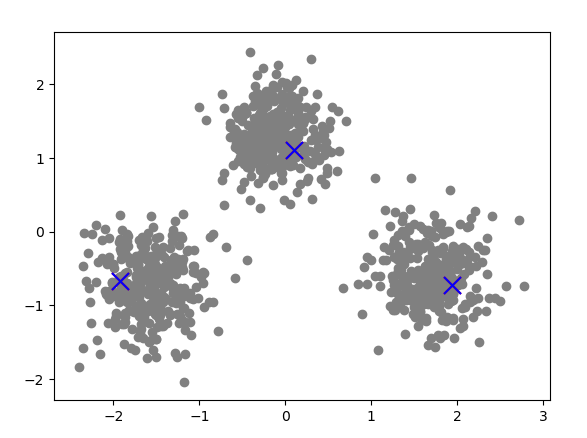
\includegraphics[width=.9\linewidth]{resources/KdSeeds.png}
			\caption{K-d tree seeds}
		\end{subfigure}%
		\begin{subfigure}{.5\textwidth}
			\centering
			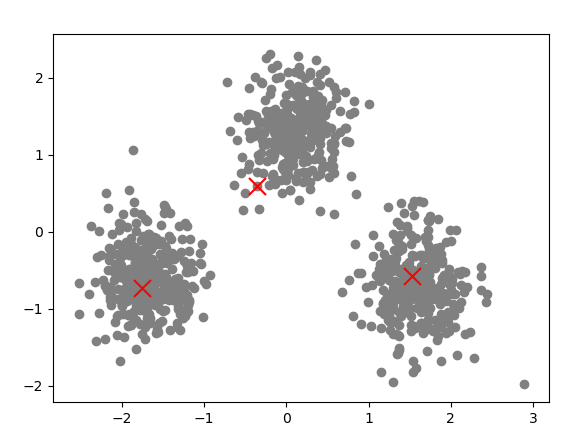
\includegraphics[width=.9\linewidth]{resources/SortAndSplitSeeds.png}
			\caption{Sort and split heuristic}
		\end{subfigure}
		\caption{Comparison of seed selection algorithms}
		\label{fig:seeds}
	\end{figure}

	The main advantage of using these seed selection strategies is the ability to get constant results. For example, the basic K-means algorithm is run using randomly selected seeds for a number of times and some results are selected in figure \ref{fig:noseeds}. For most of the runs the result is the one expected at the beginning of the experiment (the one on the left), however, one in around 5 runs obtains an undesirable clustering, due to starting with poorly selected initial seeds.
	
	\begin{figure}
	\centering
	\begin{subfigure}{.5\textwidth}
		\centering
		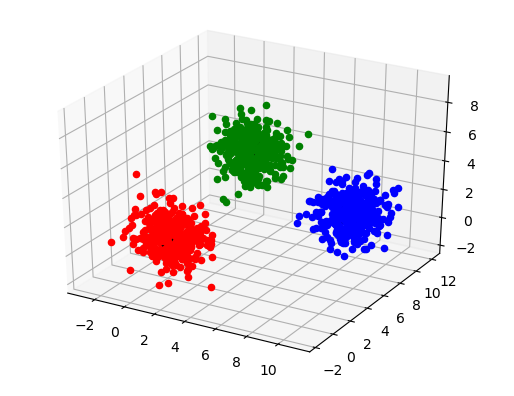
\includegraphics[width=.9\linewidth]{resources/OkKmeans.png}
		\caption{Ideal clustering}
	\end{subfigure}%
	\begin{subfigure}{.5\textwidth}
		\centering
		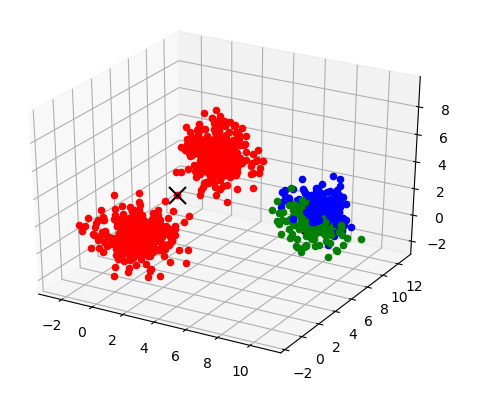
\includegraphics[width=.9\linewidth]{resources/BadKmeans.png}
		\caption{Bad starting seeds}
	\end{subfigure}
	\caption{K-Means with random seeds}
	\label{fig:noseeds}
	\end{figure}
	
	A computational performance measurement is also done by logging the execution times. Using the previous dataset the difference between basic K-Means and Enhanced K-Means is barely noticeable, only a few milliseconds. However, on a dataset of 100.000 points with 9 features each the computational times are 14 seconds for the simple algorithm and 6 for the improved one, which is already a noticeable improvement.
	
	\section{Design}
	
	\newpage
	\bibliography{references_document}
	\bibliographystyle{ieeetr}
\end{document}